%-----------------------------------------------------------------------------------------
% Autor dieser Vorlage: Stefan Macke (http://blog.macke.it Twitter: @StefanMacke) 
% Link zur Vorlage: http://f.macke.it/LaTeXVorlageFIAE 
%
% Sämtliche verwendeten Abbildungen, Tabellen und Listings stammen von Dirk Grashorn.
%
% Lizenz: Creative Commons 3.0 Namensnennung - Weitergabe unter gleichen Bedingungen
%-----------------------------------------------------------------------------------------

\documentclass[
	toc=listof, % Abbildungsverzeichnis sowie Tabellenverzeichnis in das Inhaltsverzeichnis aufnehmen
	toc=bibliography, % Literaturverzeichnis in das Inhaltsverzeichnis aufnehmen
	footnotes=multiple, % Trennen von direkt aufeinander folgenden Fußnoten
	parskip=half % vertikalen Abstand zwischen Absätzen verwenden anstatt horizontale Einrückung von Folgeabsätzen           
]{scrartcl}

\usepackage[utf8]{inputenc} % muss als erstes eingebunden werden, da Meta/Packages ggfs. Sonderzeichen enthalten

% Hinweis: der Titel muss zum Inhalt des Projekts passen und den zentralen Inhalt des Projekts deutlich herausstellen
\newcommand{\titel}{Bereitstellung einer Umgebung für Front-End-Tests und Einbindung in das Continuous-Delivery System Go}
\newcommand{\untertitel}{}

\newcommand{\autor}{Tom Zimmerlinkat}
\newcommand{\kompletterTitel}{\titel{} -- \untertitel}
\newcommand{\pruefungstermin}{Sommer 2015}
\newcommand{\ort}{Berlin}
\newcommand{\abgabetermin}{27.05.2015}
\newcommand{\ausbildungsberuf}{Fachinformatiker für Anwendungsentwicklung}
\newcommand{\betreff}{Dokumentation zur betrieblichen Projektarbeit}
%\newcommand{\logo}{LogoBetrieb.pdf}
\newcommand{\logo}{mdlogocrop.png}
 % Metadaten zu diesem Dokument (Autor usw.)
% Anpassung an Landessprache ---------------------------------------------------
\usepackage[ngerman]{babel}

% Umlaute ----------------------------------------------------------------------
%   Umlaute/Sonderzeichen wie äüöß direkt im Quelltext verwenden (CodePage).
%   Erlaubt automatische Trennung von Worten mit Umlauten.
% ------------------------------------------------------------------------------
\usepackage[T1]{fontenc}
\usepackage{textcomp} % Euro-Zeichen etc.

% Schrift ----------------------------------------------------------------------
\usepackage{lmodern} % bessere Fonts
\usepackage{relsize} % Schriftgröße relativ festlegen

% Tabellen ---------------------------------------------------------------------
\PassOptionsToPackage{table}{xcolor}
\usepackage{tabularx}
% für lange Tabellen
\usepackage{longtable}
\usepackage{array}
\usepackage{ragged2e}
\usepackage{lscape}
\newcolumntype{w}[1]{>{\raggedleft\hspace{0pt}}p{#1}} % Spaltendefinition rechtsbündig mit definierter Breite

% Grafiken ---------------------------------------------------------------------
\usepackage[dvips,final]{graphicx} % Einbinden von JPG-Grafiken ermöglichen
\usepackage{graphics} % keepaspectratio
\usepackage{floatflt} % zum Umfließen von Bildern
\graphicspath{{Bilder/}} % hier liegen die Bilder des Dokuments

% Sonstiges --------------------------------------------------------------------
\usepackage{amsmath,amsfonts} % Befehle aus AMSTeX für mathematische Symbole
\usepackage{enumitem} % anpassbare Enumerates/Itemizes
\usepackage{xspace} % sorgt dafür, dass Leerzeichen hinter parameterlosen Makros nicht als Makroendezeichen interpretiert werden

\usepackage{makeidx} % für Index-Ausgabe mit \printindex
\usepackage[printonlyused]{acronym} % es werden nur benutzte Definitionen aufgelistet

% Einfache Definition der Zeilenabstände und Seitenränder etc.
\usepackage{setspace}
\usepackage{geometry}
%Toms packs


\usepackage{todonotes}
\usepackage{booktabs}



% Symbolverzeichnis
\usepackage[intoc]{nomencl}
\let\abbrev\nomenclature
\renewcommand{\nomname}{Abkürzungsverzeichnis}
\setlength{\nomlabelwidth}{.25\hsize}
\renewcommand{\nomlabel}[1]{#1 \dotfill}
\setlength{\nomitemsep}{-\parsep}

\usepackage{url} % URL verlinken, lange URLs umbrechen etc.
\usepackage{chngcntr} % fortlaufendes Durchnummerieren der Fußnoten
\usepackage{ifthen} % bei der Definition eigener Befehle benötigt
\usepackage{todonotes} % definiert u.a. die Befehle \todo und \listoftodos
\usepackage[square]{natbib} % wichtig für korrekte Zitierweise

% PDF-Optionen -----------------------------------------------------------------
\usepackage{pdfpages}
\pdfminorversion=5 % erlaubt das Einfügen von pdf-Dateien bis Version 1.7, ohne eine Fehlermeldung zu werfen (keine Garantie für fehlerfreies Einbetten!)
\usepackage[
    bookmarks,
    bookmarksnumbered,    
    bookmarksopen=true,
    bookmarksopenlevel=1,
    colorlinks=true,
% diese Farbdefinitionen zeichnen Links im PDF farblich aus
    linkcolor=AOBlau, % einfache interne Verknüpfungen
    anchorcolor=AOBlau,% Ankertext
    citecolor=AOBlau, % Verweise auf Literaturverzeichniseinträge im Text
    filecolor=AOBlau, % Verknüpfungen, die lokale Dateien öffnen
    menucolor=AOBlau, % Acrobat-Menüpunkte
    urlcolor=AOBlau, 
% diese Farbdefinitionen sollten für den Druck verwendet werden (alles schwarz)
    %linkcolor=black, % einfache interne Verknüpfungen
    %anchorcolor=black, % Ankertext
    %citecolor=black, % Verweise auf Literaturverzeichniseinträge im Text
    %filecolor=black, % Verknüpfungen, die lokale Dateien öffnen
    %menucolor=black, % Acrobat-Menüpunkte
    %urlcolor=black, 
%
    %backref, % Quellen werden zurück auf ihre Zitate verlinkt
    pdftex,
    plainpages=false, % zur korrekten Erstellung der Bookmarks
    pdfpagelabels=true, % zur korrekten Erstellung der Bookmarks
    hypertexnames=false, % zur korrekten Erstellung der Bookmarks
    linktocpage % Seitenzahlen anstatt Text im Inhaltsverzeichnis verlinken
]{hyperref}
% Befehle, die Umlaute ausgeben, führen zu Fehlern, wenn sie hyperref als Optionen übergeben werden
\hypersetup{
    pdftitle={\titel -- \untertitel},
    pdfauthor={\autor},
    pdfcreator={\autor},
    pdfsubject={\titel -- \untertitel},
    pdfkeywords={\titel -- \untertitel},
}


% zum Einbinden von Programmcode -----------------------------------------------
\usepackage{listings}
\usepackage{xcolor} 
\definecolor{hellgelb}{rgb}{1,1,0.9}
\definecolor{colKeys}{rgb}{0,0,1}
\definecolor{colIdentifier}{rgb}{0,0,0}
\definecolor{colComments}{rgb}{0,0.5,0}
\definecolor{colString}{rgb}{1,0,0}
\lstset{
    float=hbp,
	basicstyle=\footnotesize,
    identifierstyle=\color{colIdentifier},
    keywordstyle=\color{colKeys},
    stringstyle=\color{colString},
    commentstyle=\color{colComments},
    backgroundcolor=\color{hellgelb},
    columns=flexible,
    tabsize=2,
    frame=single,
    extendedchars=true,
    showspaces=false,
    showstringspaces=false,
    numbers=left,
    numberstyle=\tiny,
    breaklines=true,
    breakautoindent=true,
	captionpos=b,
}
\lstdefinelanguage{cs}{
	sensitive=false,
	morecomment=[l]{//},
	morecomment=[s]{/*}{*/},
	morestring=[b]",
	morekeywords={
		abstract,event,new,struct,as,explicit,null,switch
		base,extern,object,this,bool,false,operator,throw,
		break,finally,out,true,byte,fixed,override,try,
		case,float,params,typeof,catch,for,private,uint,
		char,foreach,protected,ulong,checked,goto,public,unchecked,
		class,if,readonly,unsafe,const,implicit,ref,ushort,
		continue,in,return,using,decimal,int,sbyte,virtual,
		default,interface,sealed,volatile,delegate,internal,short,void,
		do,is,sizeof,while,double,lock,stackalloc,
		else,long,static,enum,namespace,string},
}
\lstdefinelanguage{natural}{
	sensitive=false,
	morecomment=[l]{/*},
	morestring=[b]",
	morestring=[b]',
	alsodigit={-,*},
	morekeywords={
		DEFINE,DATA,LOCAL,END-DEFINE,WRITE,CALLNAT,PARAMETER,USING,
		IF,NOT,END-IF,ON,*ERROR-NR,ERROR,END-ERROR,ESCAPE,ROUTINE,
		PERFORM,SUBROUTINE,END-SUBROUTINE,CONST,END-FOR,END,FOR,RESIZE,
		ARRAY,TO,BY,VALUE,RESET,COMPRESS,INTO,EQ},
}
\lstdefinelanguage{php}{
	sensitive=false,
	morecomment=[l]{/*},
	morestring=[b]",
	morestring=[b]',
	alsodigit={-,*},
	morekeywords={
		abstract,and,array,as,break,case,catch,cfunction,class,clone,const,
		continue,declare,default,do,else,elseif,enddeclare,endfor,endforeach,
		endif,endswitch,endwhile,extends,final,for,foreach,function,global,
		goto,if,implements,interface,instanceof,namespace,new,old_function,or,
		private,protected,public,static,switch,throw,try,use,var,while,xor
		die,echo,empty,exit,eval,include,include_once,isset,list,require,
		require_once,return,print,unset},
}
 % verwendete Packages
% Seitenränder -----------------------------------------------------------------
\setlength{\topskip}{\ht\strutbox} % behebt Warnung von geometry
\geometry{a4paper,left=20mm,right=20mm,top=25mm,bottom=35mm}

\usepackage[
	automark, % Kapitelangaben in Kopfzeile automatisch erstellen
	headsepline, % Trennlinie unter Kopfzeile
	ilines % Trennlinie linksbündig ausrichten
]{scrpage2}

% Kopf- und Fußzeilen ----------------------------------------------------------
\pagestyle{scrheadings}
\newcommand{\chapterpagestyle}{scrheadings}
\clearscrheadfoot

% Kopfzeile
\renewcommand{\headfont}{\normalfont} % Schriftform der Kopfzeile
\ihead{\large{\textsc{\titel}}\\ \textit{\headmark}}
%\ihead{\large{\textsc{\titel}}\\ \small{\untertitel} \\[2ex] \textit{\headmark}}
\chead{}
\ohead{\includegraphics[scale=0.15]{\logo}}
\setlength{\headheight}{15mm} % Höhe der Kopfzeile
%\setheadwidth[0pt]{textwithmarginpar} % Kopfzeile über den Text hinaus verbreitern (falls Logo den Text überdeckt) 

% Fußzeile
\ifoot{\copyright\ \autor}
\cfoot{}
\ofoot{\pagemark}

\onehalfspacing % Zeilenabstand 1,5 Zeilen
\frenchspacing % erzeugt ein wenig mehr Platz hinter einem Punkt 

% Schusterjungen und Hurenkinder vermeiden
\clubpenalty = 10000
\widowpenalty = 10000 
\displaywidowpenalty = 10000

% Quellcode-Ausgabe formatieren
\lstset{numbers=left, numberstyle=\tiny, numbersep=5pt, breaklines=true}
\lstset{emph={square}, emphstyle=\color{red}, emph={[2]root,base}, emphstyle={[2]\color{blue}}}

\counterwithout{footnote}{section} % Fußnoten fortlaufend durchnummerieren
\setcounter{tocdepth}{\subsubsectionlevel} % im Inhaltsverzeichnis werden die Kapitel bis zum Level der subsubsection übernommen
\setcounter{secnumdepth}{\subsubsectionlevel} % Kapitel bis zum Level der subsubsection werden nummeriert

% Aufzählungen anpassen
\renewcommand{\labelenumi}{\arabic{enumi}.}
\renewcommand{\labelenumii}{\arabic{enumi}.\arabic{enumii}.}
\renewcommand{\labelenumiii}{\arabic{enumi}.\arabic{enumii}.\arabic{enumiii}}

% Tabellenfärbung:
%\definecolor{heading}{rgb}{0.475,0.647,0.082}
\definecolor{heading}{rgb}{0.647,0.729,0.37}
\definecolor{odd}{rgb}{0.9,0.9,0.9}
\definecolor{gragreen}{rgb}{0.737,0.89,0.23}
%\definecolor{gragreen}{rgb}{0.52,0.667,0}
\definecolor{dropdown}{rgb}{0.431,0.49,0.6}
 % Definitionen zum Aussehen der Seiten
% Abkürzungen, ggfs. mit korrektem Leerraum 
\newcommand{\bs}{$\backslash$\xspace}
\newcommand{\bspw}{bspw.\xspace}
\newcommand{\bzw}{bzw.\xspace}
\newcommand{\ca}{ca.\xspace}
\newcommand{\dahe}{\mbox{d.\,h.}\xspace}
\newcommand{\etc}{etc.\xspace}
\newcommand{\eur}[1]{\mbox{#1\,\texteuro}\xspace}
\newcommand{\evtl}{evtl.\xspace}
\newcommand{\ggfs}{ggfs.\xspace}
\newcommand{\Ggfs}{Ggfs.\xspace}
\newcommand{\gqq}[1]{\glqq{}#1\grqq{}}
\newcommand{\inkl}{inkl.\xspace}
\newcommand{\insb}{insb.\xspace}
\newcommand{\ua}{\mbox{u.\,a.}\xspace}
\newcommand{\usw}{usw.\xspace}
\newcommand{\Vgl}{Vgl.\xspace}
\newcommand{\zB}{\mbox{z.\,B.}\xspace}

% Befehle für häufig anfallende Aufgaben
\newcommand{\Abbildung}[1]{Abbildung~\ref{fig:#1}}
\newcommand{\Anhang}[1]{Anhang~\ref{#1}: \nameref{#1} auf S.~\pageref{#1}}
\newcommand{\includegraphicsKeepAspectRatio}[2]{\includegraphics[width=#2\textwidth,height=#2\textheight,keepaspectratio]{#1}}
\newcommand{\Zitat}[2][\empty]{\ifthenelse{\equal{#1}{\empty}}{\citep{#2}}{\citep[#1]{#2}}}
\newcommand{\Autor}[1]{\textsc{#1}} % zum Ausgeben von Autoren
\newcommand{\itemd}[2]{\item{\textbf{#1}}\\{#2}} % erzeugt ein Listenelement mit fetter Überschrift

% fügt Tabellen aus einer TEX-Datei ein
\newcommand{\tabelle}[3] % Parameter: caption, label, file
{\begin{table}[htbp]
\centering
\singlespacing
\input{Tabellen/#3}
\caption{#1}
\label{#2}
\end{table}}

\newcommand{\tabelleAnhang}[1] % Parameter: file
{\begin{center}
\singlespacing
\input{Tabellen/#1}
\end{center}}

% einfaches Wechseln der Schrift, z.B.: \changefont{cmss}{sbc}{n}
\newcommand{\changefont}[3]{\fontfamily{#1} \fontseries{#2} \fontshape{#3} \selectfont}

% Verwendung analog zu \includegraphics
\newlength{\myx} % Variable zum Speichern der Bildbreite
\newlength{\myy} % Variable zum Speichern der Bildhöhe
\newcommand\includegraphicstotab[2][\relax]{%
% Abspeichern der Bildabmessungen
\settowidth{\myx}{\includegraphics[{#1}]{#2}}%
\settoheight{\myy}{\includegraphics[{#1}]{#2}}%
% das eigentliche Einfügen
\parbox[c][1.1\myy][c]{\myx}{%
\includegraphics[{#1}]{#2}}%
}

\definecolor{AOBlau}{rgb}{0, 0.28, 0.56}

% verschiedene Befehle um Wörter semantisch auszuzeichnen ----------------------
\newcommand{\Index}[2][\empty]{\ifthenelse{\equal{#1}{\empty}}{\index{#2}#2}{\index{#1}#2}}
\newcommand{\Fachbegriff}[2][\empty]{\ifthenelse{\equal{#1}{\empty}}{\textit{\Index{#2}}}{\textit{\Index[#1]{#2}}}}
\newcommand{\NeuerBegriff}[2][\empty]{\ifthenelse{\equal{#1}{\empty}}{\textbf{\Index{#2}}}{\textbf{\Index[#1]{#2}}}}

\newcommand{\Ausgabe}[1]{\texttt{#1}}
\newcommand{\Eingabe}[1]{\texttt{#1}}
\newcommand{\Code}[1]{\texttt{#1}}
\newcommand{\Datei}[1]{\texttt{#1}}

\newcommand{\Assembly}[1]{\textsf{#1}}
\newcommand{\Klasse}[1]{\textsf{#1}}
\newcommand{\Methode}[1]{\textsf{#1}}
\newcommand{\Attribut}[1]{\textsf{#1}}

\newcommand{\Datentyp}[1]{\textsf{#1}}
\newcommand{\XMLElement}[1]{\textsf{#1}}
\newcommand{\Webservice}[1]{\textsf{#1}}

\newcommand{\Refactoring}[1]{\Fachbegriff{#1}}
\newcommand{\CodeSmell}[1]{\Fachbegriff{#1}}
\newcommand{\Metrik}[1]{\Fachbegriff{#1}}
\newcommand{\DesignPattern}[1]{\Fachbegriff{#1}} % eigene allgemeine Befehle, die z.B. die Arbeit mit LaTeX erleichtern
% Tabellen, die den Zwischenstand nach einer Projektphase verdeutlichen
\newcommand{\Zwischenstand}[2]{\subsection{Zwischenstand}Tabelle~\ref{tab:#2} zeigt den Zwischenstand nach der #1.\tabelle{Zwischenstand nach der #1}{tab:#2}{#2.tex}}

% Abkürzungen
\newcommand{\Versis}{\textsc{Versis}\xspace}
\newcommand{\NI}{NatInfo\xspace}
\newcommand{\AO}{\textsc{Alte Oldenburger} Krankenversicherung\xspace}

\newcommand{\QuelleLiegtBei}{\footnote{Das Dokument kann unter \url{http://f.macke.it/LaTeXVorlageFIAEQuellen} heruntergeladen werden.}\xspace} % eigene projektspezifische Befehle, z.B. Abkürzungen usw.

\begin{document}
\thispagestyle{plain}
\begin{titlepage}

\begin{center}

\includegraphics[scale=0.25]{LogoIHK.pdf}\\[1ex]
\Large{Abschlussprüfung \pruefungstermin}\\[3ex]

\Large{\ausbildungsberuf}\\
\LARGE{\betreff}\\[4ex]

\huge{\textbf{\titel}}\\[1.5ex]
%\Large{\textbf{\untertitel}}\\[4ex]

\normalsize
Abgabetermin: \ort, den \abgabetermin\\[3em]
\textbf{Prüfungsbewerber:}\\
\autor\\
Eisenbahnstr. 129\\
14542 Werder\\[5ex]

\includegraphics{\logo}\\[2ex]
%
\includegraphics[scale=0.25]{mdlogo.jpg}\\[1ex]
\textbf{Ausbildungsbetrieb:}\\
\textsc{mobilcom-debitel} GmbH\\
Hollerstr. 126\\
24782 Büdelsdorf\\[5em]
\end{center}

\small
\noindent
-
\end{titlepage}
\clearpage

% kann nach dem Lesen entfernt werden
\pagenumbering{Alph}
%----!important----remove before release!
%----!important----remove before release!
%\thispagestyle{plain}


\begin{center}
\Large{Disclaimer}
Dieses Dokument ist eine Vorabversion und sollte nicht zur
Bewertung verwendet werden.\\Sollten sie irrtümlich diese Version
erhalten haben melden sie sich bitte unverzüglich beim Autor.\\\autor
\\
\Large{$\top W Z $}
\end{center}
\clearpage

\small
\noindent
-


%----!important----remove before release!
%----!important----remove before release!

% Preface --------------------------------------------------------------------
\pagenumbering{Roman}
\pdfbookmark[1]{Inhaltsverzeichnis}{toc}
\tableofcontents
\clearpage



% Inhalt ---------------------------------------------------------------------
\pagenumbering{arabic}
\input{ih.tex}


% Literatur ------------------------------------------------------------------
%\clearpage
%\renewcommand{\refname}{Literaturverzeichnis}
%\bibliography{Bibliographie}
%\bibliographystyle{Allgemein/natdin} % DIN-Stil des Literaturverzeichnisses
%\clearpage
\addsec{Eidesstattliche Erklärung}

% Hinweis: die eidesstattliche Erklärung ist ggfs. an die Richtlinie der IHK anzupassen

Ich, \autor, versichere hiermit, dass ich meine \textbf{\betreff} mit dem Thema
\begin{quote}
\textit{\kompletterTitel}
\end{quote}
selbständig verfasst und keine anderen als die angegebenen Quellen und Hilfsmittel benutzt habe, 
wobei ich alle wörtlichen und sinngemäßen Zitate als solche gekennzeichnet habe. Die Arbeit 
wurde bisher keiner anderen Prüfungsbehörde vorgelegt und auch nicht veröffentlicht.\\[6ex]

\ort, den \abgabetermin


\rule[-0.2cm]{5.5cm}{0.5pt}

\textsc{\autor} 


% Anhang ---------------------------------------------------------------------
\clearpage
\appendix
\pagenumbering{roman}
 \section{Anhang}
% \subsection{Detaillierte Zeitplanung}
% \label{app:Zeitplanung}

% \tabelleAnhang{ZeitplanungKomplett}

 \subsection{Lastenheft (Auszug)}
\label{app:Lastenheft}

Es folgt ein Auszug aus dem Lastenheft mit Fokus auf die Anforderungen:

Die Anforderungen orientieren sich an einem minimalen Testszenario, der
Bestellung eines Produkts im Webshop.

\textbf{Testszenario}:

\begin{itemize}
\itemsep1pt\parskip0pt\parsep0pt
\item
  Seite des Shop aufrufen
\item
  prüfen ob richtige Seite
\item
  Anmeldeformular finden
\item
  einloggen
\item
  Produktseite aufrufen
\item
  Produkt in den Warenkorb legen
\item
  zum Warenkorb navigieren
\item
  Adresse auswählen
\item
  Bezahlen
\item
  Bestellung abschicken.
\end{itemize}

\textbf{Testfähigkeiten}

Daraus abgeleitet muss ein Test folgende Anforderungen erfüllen:

\begin{itemize}
\itemsep1pt\parskip0pt\parsep0pt
\item
  Seiten aufrufen
\item
  HTTP und HTTPS Verbindungen
\item
  Überprüfen ob Element auf Seite vorhanden.
\item
  Navigieren der Seite und Identifizierung von Elementen mit Hilfe von
  XPATH\footnote{XML Abfragesprache, um Teile eines XML-Dokumentes zu
    adressieren}, CSS-Selektoren \footnote{Syntax in Cascading
    Stylesheets, um Teile eines HTML-Dokumentes zu adressieren } oder
  dem Inhalt von Elementen
\item
  Website anhand von Links navigieren
\item
  Javascript ausführen
\item
  Formulare wie z.B. das Anmeldeformular oder das Adressformular im Shop
  im Browser ausfüllen und absenden. Der Test soll die gleiche
  Javascript-basierte Validierung erfahren wie der Nutzer auch. Der
  einfache Versand von vorausgefüllten HTTP-POST-Request genügt nicht. 
\item
  Logging des Testergebnis mit Ausgabe von Kommentaren im Testskript
\end{itemize}

\textbf{Umgebungsfähigkeiten}

Zusätzlich zu den Fähigkeiten der Tests gibt es Anforderungen an die
Testumgebung und ihre Integration. :

\begin{itemize}
\itemsep1pt\parskip0pt\parsep0pt
\item
  Die Testmgebung muss auf mindestens einer der bestehenden
  Serverumgebungen lauffähig sein (Syseleven: Gentoo Linux, md
  Rechenzentrum Düsseldorf: Suse Linux oder Ubuntu, Amazon EC2 virtuelle
  Instanz mit Ubuntu)
\item
  Die Testläufe müssen aus dem CI/CD System \emph{Go} ausgelöst werden
  können.
\item
  Die Testumgebung muss Erfolg oder Misserfolg eines Tests als
  Rückgabewert liefern können.
\item
  Die Testumgebung muss im Fehlerfall oder auf explizite Anweisung
  Screenshots der Seite erstellen
\item
  Es können Testbedingungen für den Test bereitgestellt werden. z.B. in
  Form von Datenbankabfragen die vorab Testnutzer und Testdaten anlegen
  oder wiederherstellen.
\item
  Es können Parameter aus dem CI/CD-System an das Testsystem zur
  verfeinerten Steuerung der Testtiefe oder Auswahl von Testobjekten
  weiter gereicht werden.
\item
  Es muss eine Historie von Testergebnissen und Artefakten und Testlogs
  von alten Testläufen aufbewahrt werden
\item
  Es müssen aktuelle Testskripte aus der Versionsverwaltung
  \emph{svn.gravis.de} ausgecheckt werden können
\item
  Eine Testsuite muss aus dem CI/CD System heraus gewählt werden können.
\item
  Es muss eine maschinenlesbare Auswertung von Tests erstellt werden.
  Hierfür wird das XUNIT Format bevorzugt.
\end{itemize}

 \clearpage
 \section{Pflichtenheft (Auszug)}\label{pflichtenheft-auszug}

\begin{quote}
//ich bin ein Lösungskonzept, quasi, glaube ich
\end{quote}

Im folgenden Auszug aus dem Pflichtenheft wird die geplante Umsetzung
der im Lastenheft definierten Anforderungen beschrieben

\subsubsection{Umsetzung der Anforderungen
Test-Runtime}\label{umsetzung-der-anforderungen-test-runtime}

\begin{quote}
// Todo: habe wohl manchmal ghost und ghostjs geschrieben, ist falsch,
das ist was anderes. Alles so Gespensterworte, da kommt man
durcheinander.
\end{quote}

\begin{itemize}
\item
  Als Browser der Testumgebung wird PhantomJS\footnote{phantomjs.org/headless-testing.html}
  gewählt. Die Installation erfolgt über die Paketverwaltung der
  jeweiligen Distribution, das heißt portage\footnote{packages.gentoo.org/package/sys-apps/portage}
  für Gentoo, APT\footnote{wiki.ubuntuusers.de/APT} auf Ubuntu,
  brew\footnote{brew.sh} auf MacOS.
  \texttt{ich\ möchte\ das\ extra\ ansprechen,\ muss\ aber\ nicht\ im\ Pflichtenheft\ sein\ -\textgreater{}}
  Es werden die Binärdateien aus den jeweiligen Repositories genutzt.
  Zum Projektzeitpunkt wird PhantomJS 1.9.8 verteil. PhantomJS sollte
  nicht selbst kompiliert werden da es enorm viele Abhängigkeiten hat,
  was viele zusätzliche Fehlerquellen mit sich ziehen kann, und weil der
  Kompiliervorgang auch einem modernen Applikationsserver mehrere
  Stunden dauert. Da PhantomJS 2.0.0 auf dem Macintosh noch nicht
  startet und für linux nicht compiliert und die Tests und Testsuiten
  auf solchen Rechnern erstellt werden sollen, ist es empfohlen bei der
  stabilen Version 1.9.8 zu bleiben die sowohl unter Linux als auch Mac
  und Windows eingesetzt werden kann.

  \#asert you are on a 32 bit
  system\texttt{cd\ /usr/local/share\ sudo\ wget\ https://bitbucket.org/ariya/phantomjs/downloads/phantomjs-1.9.8-linux-i686.tar.bz2\ sudo\ tar\ xjf\ phantomjs-1.9.8-linux-i686.tar.bz2\ sudo\ ln\ -s\ /usr/local/share/phantomjs-1.9.8-linux-i686/bin/phantomjs\ /usr/local/share/phantomjs\ sudo\ ln\ -s\ /usr/local/share/phantomjs-1.9.8-linux-i686/bin/phantomjs\ /usr/local/bin/phantomjs\ sudo\ ln\ -s\ /usr/local/share/phantomjs-1.9.8-linux-i686/bin/phantomjs\ /usr/bin/phantomjs}
\item
  Als Test Runtime wird casperJS\footnote{} genutzt, es steht ebenfalls
  in den gängigen Repositories zur Verfügung und muss nicht selbst
  kompiliert werden. \textgreater{}//ätsch, in portage nicht, da muss
  man das selber auschecken. code steht hier temporär

  \$ git clone git://github.com/n1k0/casperjs.git \$ cd casperjs \$ ln
  -sf \texttt{pwd}/bin/casperjs /usr/local/bin/casperjs
\item
  casperJS wird mit einem \emph{tester} Modul ausgeliefert, welches für
  Unit- und funktionale Tests genutzt werden kann und eine API zur
  Verfügung stellt welche
  \texttt{vollständig?\ -\ muss\ ich\ das\ beweisen?} den Anforderungen
  an Testfähigkeiten aus dem Lastenheft genügt.
\item
  Tests werden in Javascript oder Coffeescript\footnote{coffescript.org
    coffescript ist eine Sprache die nach Javascript, genauer ECMAScript
    3, transcompiliert werden kann. Sie inspiriert sich von anderen
    Programmiersprachen wie Ruby oder Python und ist als syntactic sugar
    für JavaScript zu verstehen * Eine Ausgabe erfolgt von CasperJS}:
  geschrieben und nutzen die Funktionalität des \emph{tester} Modul von
  GhostJS zum abtasten der jeweiligen Seite und Funktionalität des
  \emph{utilis} Modul zum verarbeiten der Eingabeparameter und
  Ausgabe.\\Eine Aufnahme von Testabläufen ist mit den der
  Chrome-extension \emph{resurrectio}\footnote{https://github.com/ebrehault/resurrectio}
  möglich, diese gibt nach der Ausgabe den Quellcode eines Test als
  Javascript aus. \emph{resurrectio} wird seid 2013 nicht mehr gewartet
  sodass damit erstellte Tests nicht den vollen Funktionsumfang von
  Ghostjs \texttt{\$currentversion\ \ ,\ 1.0\ beta\ 3} ausnutzen können.
\item
  Test werden als JavaScript-Dateien gespeichert
\end{itemize}

Bildschrimfotos werden wie folgt erstellt.
https://github.com/casperjs/responsive-screenshots

\subsubsection{Umsetzung der Anforderungen Integration ins CI/CD
System}\label{umsetzung-der-anforderungen-integration-ins-cicd-system}

\begin{itemize}
\item
  Die Flusskontrolle \texttt{Die\ Logik\ ?} für Deployment- und
  Integrationsprozesse wird definiert mit Hilfe von ANT Skripten.
  Einzelne Aufgaben werden in sogenannte Pipelines verpackt.
  \texttt{Dieser\ Punkt\ kommt\ in\ den\ Flusstext,\ nicht\ Pflichtenheft}
\item
  Es wird in Go eine neue Pipelinegruppe angelegt mit je einer Pipeline
  pro zu testender Serverumgebung. Hier sind es 3 für das
  \emph{Integration}, \emph{Stage} und \emph{Echt}‌system.\\ Dazu werden
  neue Tags \texttt{XML-Knoten?} für Pipelines in die \texttt{go.xml}
  eingefügt. Der teaminternen Nomenklatur folgend heißen die Pipelines
  dann etwas ``UI.Test.ghostjs'' und ``UL.Test.ghostjs''
  \textgreater{}// Todo: Name klären
\item
  Es wird eine neue ghostjs.xml Datei erstellt die sämtliche ANT-Targets
  enthalten wird die für Regressionstests notwendig sind. Diese
  beinhalten u.a. :

  \begin{itemize}
  \itemsep1pt\parskip0pt\parsep0pt
  \item
    Auschecken aktueller Tests und Konfigurationsdateien aus der
    Versionsverwaltung ``svn.gravis.de/testing/trunk/ghostjs'' in das
    Basisverzeichnis der aktuellen Pipeline
  \item
    Vor-
  \item
    und nachbereitende Datenbankabfragen die Nutzerdaten von und für die
    Testnutzer der Regressionstests wie etwas Adressänderungen oder das
    löschen von Testkonten.
  \item
    Das Auslösen der Test
  \item
    Das Abholen und Aufbereitung der Testartefakte
  \item
    Die Auswertung der Testergebnisse
  \end{itemize}
\item
  Umgebungsvariablen werden in Go vergeben, die Basispfade für
  Testdateien und Artefakte festlegen, sowie Zugangsdaten für vor- und
  nachbereitende Datenbankzugriffe
\item
  Auf allen von Go verwalteten Servern muss ein ``Go-Agent'' ausgeführt
  werden. Dieser nimmt dann Arbeitsanweisungen von CI/CD System, aus den
  Pipelines entgegen und führt diese aus. Der Agent auf dem Server für
  Regressionstest muss in Go registriert werden.
\item
  Den Agenten muss eine oder mehrere Ressource(n) als Merkmal
  hinzugefügt werden

  \texttt{\textless{}agents\textgreater{}\ \ \ \ \ \textless{}agent\textgreater{}\ \ \ \ \ \ \ \ \ \textless{}name\textgreater{}mdsonline.stage.gravis.de.app2\textless{}/name\textgreater{}\ \ \ \ \ \ \ \ \ \textless{}ressources\textgreater{}stage\textless{}/ressources\textgreater{}\ \ \ \ \ \textless{}/agent\textgreater{}\ \textless{}agents\textgreater{}}
\item
  Zuweisung der ausführenden Ressource zu den jeweiligen Testing
  Pipelines.

  \texttt{\textless{}pipeline\textgreater{}\ \ \ \ \ \textless{}name\textgreater{}G.UI.testing.ghostjs\textless{}/name\textgreater{}\ \ \ \ \ \textless{}ressources\textgreater{}manager,stage\textless{}/ressources\textgreater{}\ \ \ \textless{}/pipeline\textgreater{}}
\item
  Das Auslösen der Test erfolgt über ein Unix-Shellkommando in einem
  ANT-Target. Hierbei wird casperJS mit Argumenten und Parametern
  aufgerufen. Hierbei können die Testtiefe als auch weitere Parameter
  übergebenwerden, etwa die gezielte Angebe von Suchtermini
  \texttt{\$ENV\_searchterms} oder Artikelnummern
  \texttt{\$ENV\_testporducts} die in die Test mit einbezogen werden
  sollen. Diese werden in Go als Umgebungsvariablen definiert und dann
  in das Unix-Shellkommando eingefügt.
  \texttt{casperjs\ Test\ pfad/zu/tests/*.js\ -\/-testdebth=\{\$ENV\_testdebth\}\ -\/-testproducts=\{\$ENV\_testporducts\}\ -\/-searchterms=\{\$ENV\_searchterms\}}.
  Damit ist bereits aus der Weboberfläche des CI/CD System eine hohe
  Anpassungsfähigkeit der Tests gewährleistet. Der Testleiter kann
  hierdurch ohne umständliche Code-Anpassungen die Testtiefe einstellen.
\item
  Es wird eine ``Pre-run'' Konfigurationsdatei für CasperJS die
  Zugangsdaten und wiederkehrende Prozeduren enthält sowie die
  Kommandozeilenparameter und -argumente aufbereitet und den folgenden
  Test in Variablen zur Verfügung stellt.
\item
  Ort für Artefakte bereiten
\item
  Ausgabe von Artefakten definieren (Screenshot)
\item
  Ausgabe von Artefakten definieren (XUnit-log)
\item
  Ausgabe von Artefakten definieren (Verbose Ausgabe von Casper
  \texttt{in\ Datei\ piepen?\ Kann\ ich\ ANSI-Farben\ behalten?})
\item
  \texttt{XUNIT-log\ schönen/aufbereiten?\ PHPUnit\ hat\ an\ dieser\ Stelle\ eine\ kleine\ Reportwebpage\ erstellt\ -\textgreater{}\ Will\ ich\ das,\ brauche\ ich\ das?}
\item
  Rückgabewerte an Go konkretisieren.
  \texttt{Schlägt\ die\ Pipeline\ fehl\ nur\ weil\ ein\ Test\ Fehlgeschlagen\ ist?}
\end{itemize}

 \clearpage

% \subsection{Use Case-Diagramm}
% \label{app:UseCase}
% Use Case-Diagramme und weitere \acs{UML}-Diagramme kann man auch direkt mit \LaTeX{} zeichnen, siehe \zB \url{http://metauml.sourceforge.net/old/usecase-diagram.html}.
% \begin{figure}[htb]
% \centering
% \includegraphicsKeepAspectRatio{UseCase.pdf}{0.7}
% \caption{Use Case-Diagramm}
% \end{figure}

% \subsection{Pflichtenheft (Auszug)}
\label{app:Pflichtenheft}

\subsubsection*{Zielbestimmung}

\begin{enumerate}[itemsep=0em,partopsep=0em,parsep=0em,topsep=0em]
\item Musskriterien % Wikipedia: für das Produkt unabdingbare Leistungen, die in jedem Fall erfüllt werden müssen
	\begin{enumerate}
	\item Modul-Liste: Zeigt eine filterbare Liste der Module mit den dazugehörigen Kerninformationen sowie Symbolen zur Einhaltung des Entwicklungsprozesses an
		\begin{itemize}
		\item In der Liste wird der Name, die Bibliothek und Daten zum Source und Kompilat eines Moduls angezeigt.
		\item Ebenfalls wird der Status des Moduls hinsichtlich Source und Kompilat angezeigt. Dazu gibt es unterschiedliche Status-Zeichen, welche symbolisieren in wie weit der Entwicklungsprozess eingehalten wurde \bzw welche Schritte als nächstes getan werden müssen. So gibt es \zB Zeichen für das Einhalten oder Verletzen des Prozesses oder den Hinweis auf den nächsten zu tätigenden Schritt. 
		\item Weiterhin werden die Benutzer und Zeitpunkte der aktuellen Version der Sourcen und Kompilate angezeigt. Dazu kann vorher ausgewählt werden, von welcher Umgebung diese Daten gelesen werden sollen. 
		\item Es kann eine Filterung nach allen angezeigten Daten vorgenommen werden. Die Daten zu den Sourcen sind historisiert. Durch die Filterung ist es möglich, auch Module zu finden, die in der Zwischenzeit schon von einem anderen Benutzer editiert wurden.
		\end{itemize}
	\item Tag-Liste: Bietet die Möglichkeit die Module anhand von Tags zu filtern. 
		\begin{itemize}
		\item Es sollen die Tags angezeigt werden, nach denen bereits gefiltert wird und die, die noch der Filterung hinzugefügt werden könnten, ohne dass die Ergebnisliste leer wird.
		\item Zusätzlich sollen die Module angezeigt werden, die den Filterkriterien entsprechen. Sollten die Filterkriterien leer sein, werden nur die Module angezeigt, welche mit einem Tag versehen sind.
		\end{itemize}
	\item Import der Moduldaten aus einer bereitgestellten \acs{CSV}-Datei
		\begin{itemize}
		\item Es wird täglich eine Datei mit den Daten der aktuellen Module erstellt. Diese Datei wird (durch einen Cronjob) automatisch nachts importiert.
		\item Dabei wird für jedes importierte Modul ein Zeitstempel aktualisiert, damit festgestellt werden kann, wenn ein Modul gelöscht wurde.
		\item Die Datei enthält die Namen der Umgebung, der Bibliothek und des Moduls, den Programmtyp, den Benutzer und Zeitpunkt des Sourcecodes sowie des Kompilats und den Hash des Sourcecodes.
		\item Sollte sich ein Modul verändert haben, werden die entsprechenden Daten in der Datenbank aktualisiert. Die Veränderungen am Source werden dabei aber nicht ersetzt, sondern historisiert.
		\end{itemize}
	\item Import der Informationen aus \ac{SVN}. Durch einen \gqq{post-commit-hook} wird nach jedem Einchecken eines Moduls ein \acs{PHP}-Script auf der Konsole aufgerufen, welches die Informationen, die vom \ac{SVN}-Kommandozeilentool geliefert werden, an \acs{NatInfo} übergibt.
	\item Parsen der Sourcen
		\begin{itemize}
		\item Die Sourcen der Entwicklungsumgebung werden nach Tags, Links zu Artikeln im Wiki und Programmbeschreibungen durchsucht.
		\item Diese Daten werden dann entsprechend angelegt, aktualisiert oder nicht mehr gesetzte Tags/Wikiartikel entfernt.
		\end{itemize}
	\item Sonstiges
		\begin{itemize}
		\item Das Programm läuft als Webanwendung im Intranet.
		\item Die Anwendung soll möglichst leicht erweiterbar sein und auch von anderen Entwicklungsprozessen ausgehen können.
		\item Eine Konfiguration soll möglichst in zentralen Konfigurationsdateien erfolgen.
		\end{itemize}
	\end{enumerate}
\end{enumerate}

\subsubsection*{Produkteinsatz}

\begin{enumerate}[itemsep=0em,partopsep=0em,parsep=0em,topsep=0em]
\item{Anwendungsbereiche\\
Die Webanwendung dient als Anlaufstelle für die Entwicklung. Dort sind alle Informationen für die Module an einer Stelle gesammelt. Vorher getrennte Anwendungen werden ersetzt \bzw verlinkt.}
\item{Zielgruppen\\
\NI wird lediglich von den \ac{Natural}-Entwicklern in der EDV-Abteilung genutzt.}
\item{Betriebsbedingungen\\ % Wikipedia: physikalische Umgebung des Systems, tägliche Betriebszeit, ständige Beobachtung des Systems durch Bediener oder unbeaufsichtigter Betrieb
Die nötigen Betriebsbedingungen, also der Webserver, die Datenbank, die Versionsverwaltung, das Wiki und der nächtliche Export sind bereits vorhanden und konfiguriert. Durch einen täglichen Cronjob werden entsprechende Daten aktualisiert, die Webanwendung ist jederzeit aus dem Intranet heraus erreichbar.}
\end{enumerate}


% \subsection{Datenbankmodell}
% \label{app:Datenbankmodell}
% ER-Modelle kann man auch direkt mit \LaTeX{} zeichnen, siehe \zB \url{http://www.texample.net/tikz/examples/entity-relationship-diagram/}.
% \begin{figure}[htb]
% \centering
% \includegraphicsKeepAspectRatio{database.pdf}{1}
% \caption{Datenbankmodell}
% \end{figure}
% \clearpage

% \subsection{Oberflächenentwürfe}
\label{app:Entwuerfe}
\begin{figure}[htb]
\centering
\includegraphicsKeepAspectRatio{MockupModules.pdf}{0.7}
\caption{Liste der Module mit Filtermöglichkeiten}
\end{figure}

\begin{figure}[htb]
\centering
\includegraphicsKeepAspectRatio{MockupModul.pdf}{0.7}
\caption{Anzeige der Übersichtsseite einzelner Module}
\end{figure}

\begin{figure}[htb]
\centering
\includegraphicsKeepAspectRatio{MockupTag.pdf}{0.7}
\caption{Anzeige und Filterung der Module nach Tags}
\end{figure}

% \clearpage
% \subsection{Screenshots der Anwendung}
\label{Screenshots}
\begin{figure}[htb]
\centering
\includegraphicsKeepAspectRatio{tagliste.pdf}{1}
\caption{Anzeige und Filterung der Module nach Tags}
\end{figure}
\clearpage
\begin{figure}[htb]
\centering
\includegraphicsKeepAspectRatio{modulliste.pdf}{1}
\caption{Liste der Module mit Filtermöglichkeiten}
\end{figure}
\clearpage

% \subsection{Entwicklerdokumentation}
\label{app:Doc}
\begin{center}
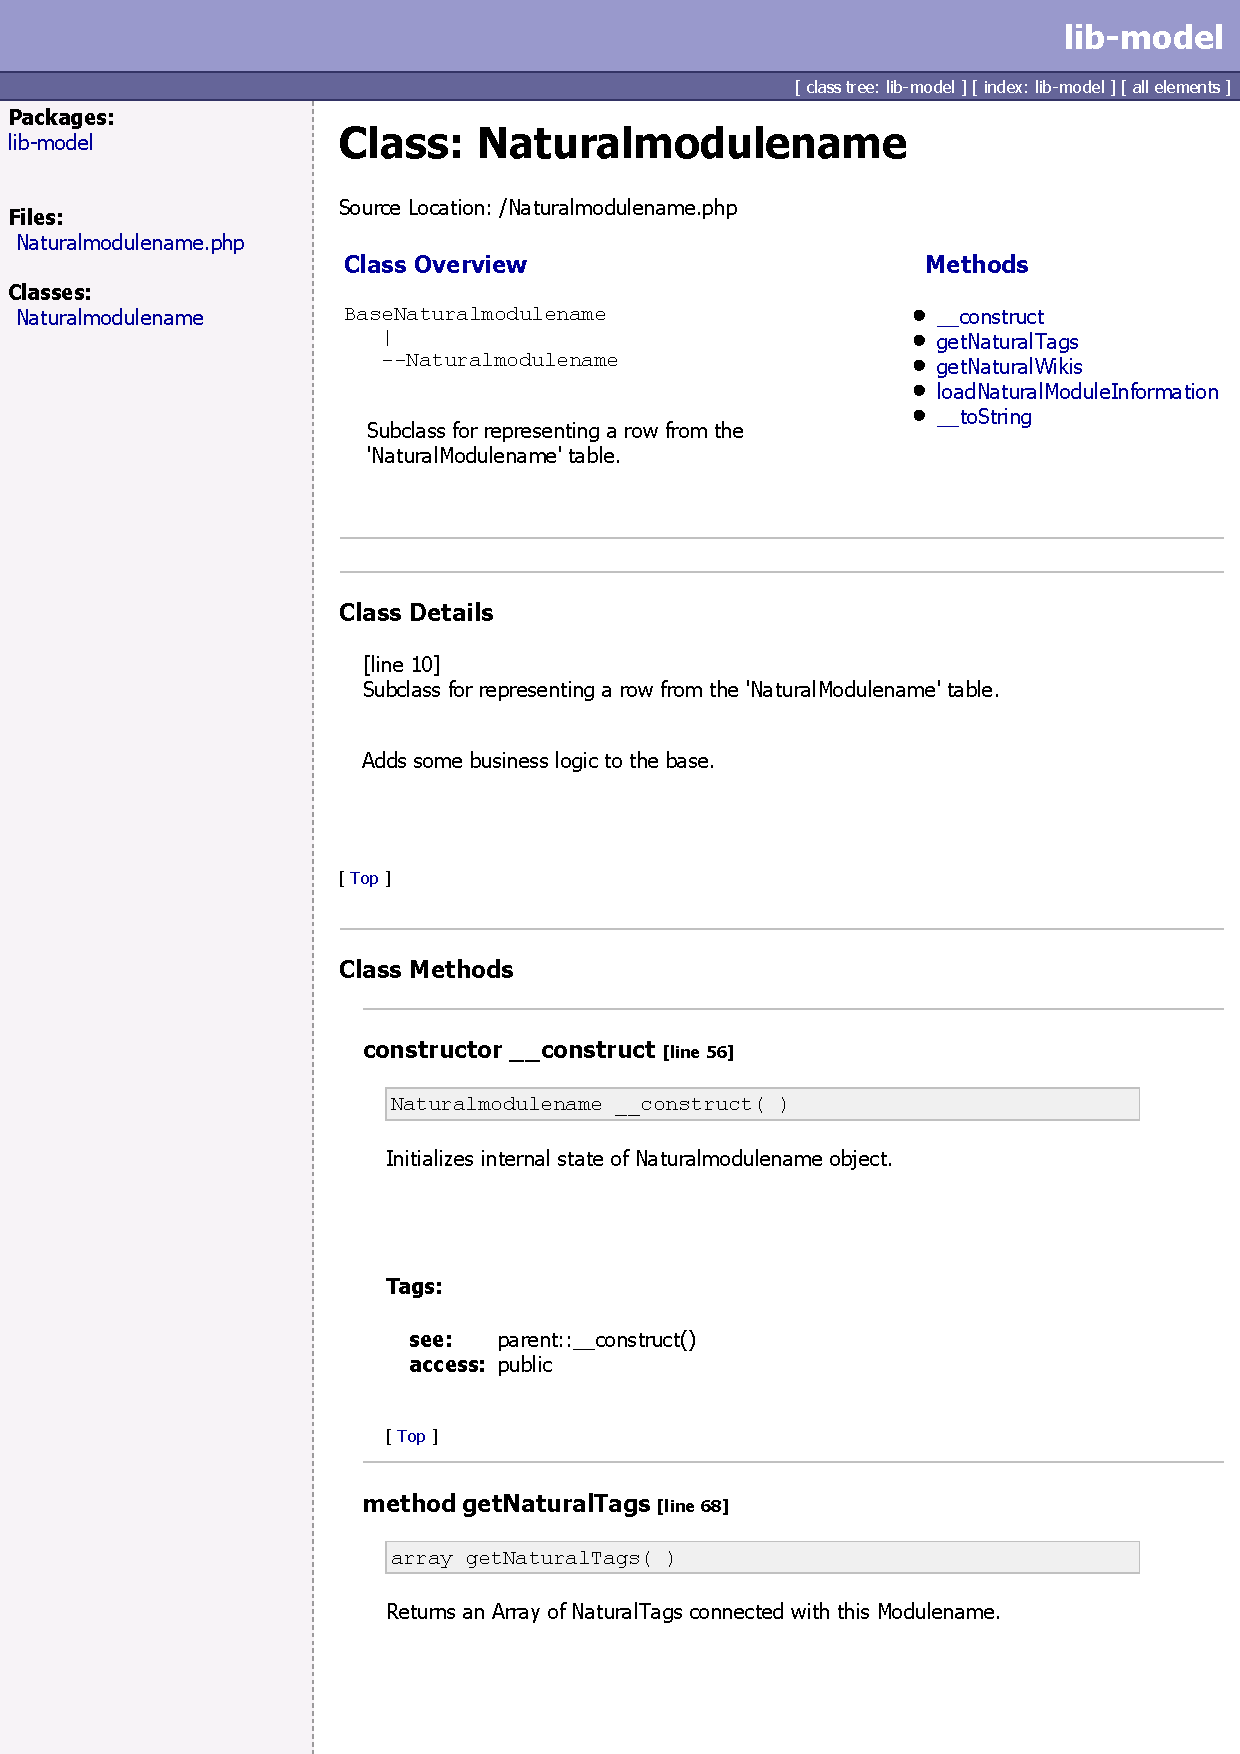
\includegraphics[page=1, width=0.9\textwidth]{doc.pdf}

\includegraphics[page=2, width=0.9\textwidth]{doc.pdf}
\end{center}

% \clearpage
% \subsection{Testfall und sein Aufruf auf der Konsole}
\label{app:Test}
\lstinputlisting[language=php]{Listings/tests.php}
\clearpage
\begin{figure}[htb]
\centering
\includegraphicsKeepAspectRatio{testcase.jpg}{1}
\caption{Aufruf des Testfalls auf der Konsole}
\end{figure}


% \subsection{Klasse: ComparedNaturalModuleInformation}
% \label{app:CNMI}
% Kommentare und simple Getter/Setter werden nicht angezeigt.
% \lstinputlisting[language=php]{Listings/cnmi.php}
% \clearpage

% \subsection{Klassendiagramm}
% \label{app:Klassendiagramm}
% Klassendiagramme und weitere \acs{UML}-Diagramme kann man auch direkt mit \LaTeX{} zeichnen, siehe \zB \url{http://metauml.sourceforge.net/old/class-diagram.html}.
% \begin{figure}[htb]
% \centering
% \includegraphicsKeepAspectRatio{Klassendiagramm.pdf}{1}
% \caption{Klassendiagramm}
% \end{figure}
% \clearpage

% \subsection{Benutzerdokumentation}
\label{app:BenutzerDoku}
Ausschnitt aus der Benutzerdokumentation:

\begin{table}[htb]
\begin{tabularx}{\textwidth}{cXX}
\rowcolor{heading}\bf{Symbol} & \bf{Bedeutung global} & \bf{Bedeutung einzeln} \\
\includegraphicstotab[]{weather-clear.png} & Alle Module weisen den gleichen Stand auf. & Das Modul ist auf dem gleichen Stand wie das Modul auf der vorherigen Umgebung. \\
\rowcolor{odd}\includegraphicstotab[]{weather-clear-night.png} & Es existieren keine Module (fachlich nicht möglich). & Weder auf der aktuellen noch auf der vorherigen Umgebung sind Module angelegt. Es kann also auch nichts übertragen werden. \\
\includegraphicstotab[]{weather-few-clouds-night.png} & Ein Modul muss durch das Übertragen von der vorherigen Umgebung erstellt werden. & Das Modul der vorherigen Umgebung kann übertragen werden, auf dieser Umgebung ist noch kein Modul vorhanden. \\
\rowcolor{odd}\includegraphicstotab[]{weather-few-clouds.png} & Auf einer vorherigen Umgebung gibt es ein Modul, welches übertragen werden kann, um das nächste zu aktualisieren. & Das Modul der vorherigen Umgebung kann übertragen werden um dieses zu aktualisieren. \\
\includegraphicstotab[]{weather-storm.png} & Ein Modul auf einer Umgebung wurde entgegen des Entwicklungsprozesses gespeichert. & Das aktuelle Modul ist neuer als das Modul auf der vorherigen Umgebung oder die vorherige Umgebung wurde übersprungen. \\
\end{tabularx}
\end{table}



%\subsection{Lastenheft (Auszug)}
\label{app:Lastenheft}

Es folgt ein Auszug aus dem Lastenheft mit Fokus auf die Anforderungen:

Die Anforderungen orientieren sich an einem minimalen Testszenario, der
Bestellung eines Produkts im Webshop.

\textbf{Testszenario}:

\begin{itemize}
\itemsep1pt\parskip0pt\parsep0pt
\item
  Seite des Shop aufrufen
\item
  prüfen ob richtige Seite
\item
  Anmeldeformular finden
\item
  einloggen
\item
  Produktseite aufrufen
\item
  Produkt in den Warenkorb legen
\item
  zum Warenkorb navigieren
\item
  Adresse auswählen
\item
  Bezahlen
\item
  Bestellung abschicken.
\end{itemize}

\textbf{Testfähigkeiten}

Daraus abgeleitet muss ein Test folgende Anforderungen erfüllen:

\begin{itemize}
\itemsep1pt\parskip0pt\parsep0pt
\item
  Seiten aufrufen
\item
  HTTP und HTTPS Verbindungen
\item
  Überprüfen ob Element auf Seite vorhanden.
\item
  Navigieren der Seite und Identifizierung von Elementen mit Hilfe von
  XPATH\footnote{XML Abfragesprache, um Teile eines XML-Dokumentes zu
    adressieren}, CSS-Selektoren \footnote{Syntax in Cascading
    Stylesheets, um Teile eines HTML-Dokumentes zu adressieren } oder
  dem Inhalt von Elementen
\item
  Website anhand von Links navigieren
\item
  Javascript ausführen
\item
  Formulare wie z.B. das Anmeldeformular oder das Adressformular im Shop
  im Browser ausfüllen und absenden. Der Test soll die gleiche
  Javascript-basierte Validierung erfahren wie der Nutzer auch. Der
  einfache Versand von vorausgefüllten HTTP-POST-Request genügt nicht. 
\item
  Logging des Testergebnis mit Ausgabe von Kommentaren im Testskript
\end{itemize}

\textbf{Umgebungsfähigkeiten}

Zusätzlich zu den Fähigkeiten der Tests gibt es Anforderungen an die
Testumgebung und ihre Integration. :

\begin{itemize}
\itemsep1pt\parskip0pt\parsep0pt
\item
  Die Testmgebung muss auf mindestens einer der bestehenden
  Serverumgebungen lauffähig sein (Syseleven: Gentoo Linux, md
  Rechenzentrum Düsseldorf: Suse Linux oder Ubuntu, Amazon EC2 virtuelle
  Instanz mit Ubuntu)
\item
  Die Testläufe müssen aus dem CI/CD System \emph{Go} ausgelöst werden
  können.
\item
  Die Testumgebung muss Erfolg oder Misserfolg eines Tests als
  Rückgabewert liefern können.
\item
  Die Testumgebung muss im Fehlerfall oder auf explizite Anweisung
  Screenshots der Seite erstellen
\item
  Es können Testbedingungen für den Test bereitgestellt werden. z.B. in
  Form von Datenbankabfragen die vorab Testnutzer und Testdaten anlegen
  oder wiederherstellen.
\item
  Es können Parameter aus dem CI/CD-System an das Testsystem zur
  verfeinerten Steuerung der Testtiefe oder Auswahl von Testobjekten
  weiter gereicht werden.
\item
  Es muss eine Historie von Testergebnissen und Artefakten und Testlogs
  von alten Testläufen aufbewahrt werden
\item
  Es müssen aktuelle Testskripte aus der Versionsverwaltung
  \emph{svn.gravis.de} ausgecheckt werden können
\item
  Eine Testsuite muss aus dem CI/CD System heraus gewählt werden können.
\item
  Es muss eine maschinenlesbare Auswertung von Tests erstellt werden.
  Hierfür wird das XUNIT Format bevorzugt.
\end{itemize}


% Formaler Anhang ----------
\clearpage
\listoffigures



\listoftables
\clearpage

\newcommand{\abkvz}{Abkürzungsverzeichnis}
\renewcommand{\nomname}{\abkvz}
\section*{\abkvz}
\markboth{\abkvz}{\abkvz}
\addcontentsline{toc}{section}{\abkvz}
% Es werden nur die Abkürzungen aufgelistet, die mit \ac definiert und auch benutzt wurden. 
%
% \acro{VERSIS}{Versicherungsinformationssystem\acroextra{ (Bestandsführungssystem)}}
% Ergibt in der Liste: VERSIS Versicherungsinformationssystem (Bestandsführungssystem)
% Im Text aber: \ac{VERSIS} -> Versicherungsinformationssystem (VERSIS)

% Hinweis: allgemein bekannte Abkürzungen wie z.B. bzw. u.a. müssen nicht ins Abkürzungsverzeichnis aufgenommen werden
% Hinweis: allgemein bekannte IT-Begriffe wie Datenbank oder Programmiersprache müssen nicht erläutert werden,
%          aber ggfs. Fachbegriffe aus der Domäne des Prüflings (z.B. Versicherung)

\begin{acronym}
	\acro{API}{Application Programming Interface}
	\acro{CI/CD}{Continuous Integration, Continuous Deployment}
	\acro{CI}{Continuous Integration}
	\acro{CD}{Continuous Deployment}
	\acro{CSS}{Cascading Style Sheets}
	\acro{CSV}{Comma Separated Value}
	\acro{Go}{Thoughtworks Go, Continuous Integration System}
	\acro{GRAVIS}{GRAVIS Computervertriebsgesellschaft mbH}
	\acro{HTML}{Hypertext Markup Language}\acused{HTML}
	\acro{IDE}{Integrated Development Environment}
	\acro{md}{mobilcom-debitel}
	\acro{Natural}[\textsc{Natural}]{Programmiersprache der Software AG}\acused{Natural}
	\acro{PHP}{PHP Hypertext Preprocessor}
	\acro{RAM}{Random Access Memory}
	\acro{SDK}{Software Development Kit}
	\acro{SQL}{Structured Query Language}
	\acro{SVN}{Subversion}
\end{acronym}

\clearpage


%credit for author of LaTeX Template
%Diese \LaTeX-Vorlage wurde von Stefan Macke\footnote{Blog des Autors: \url{http://blog.macke.it}, Twitter: \Eingabe{@StefanMacke}} entwickelt. Download-Link für diese Vorlage: \url{http://f.macke.it/LaTeXVorlageFIAE}
%license: CC-BY-SA

\end{document}
